Relacionado a la primer ejecución del algoritmo, este tomó un total de 11 épocas para lograr la convergencia, obteniendo los siguientes resultados:
\begin{itemize}
	\item Mejor individuo: $(1.2670, 1.6521)$
	\item Aptitud: $0.2907$
\end{itemize}

La Figura \ref{fig:AG_1} muestra el proceso de evolución en términos de aptitud, mientras que la Figura \ref{fig:Ev1} muestra una comparación entre los individuos durante la primer época contra los individuos de la última época.

\begin{figure}[htbp]
	\centering
	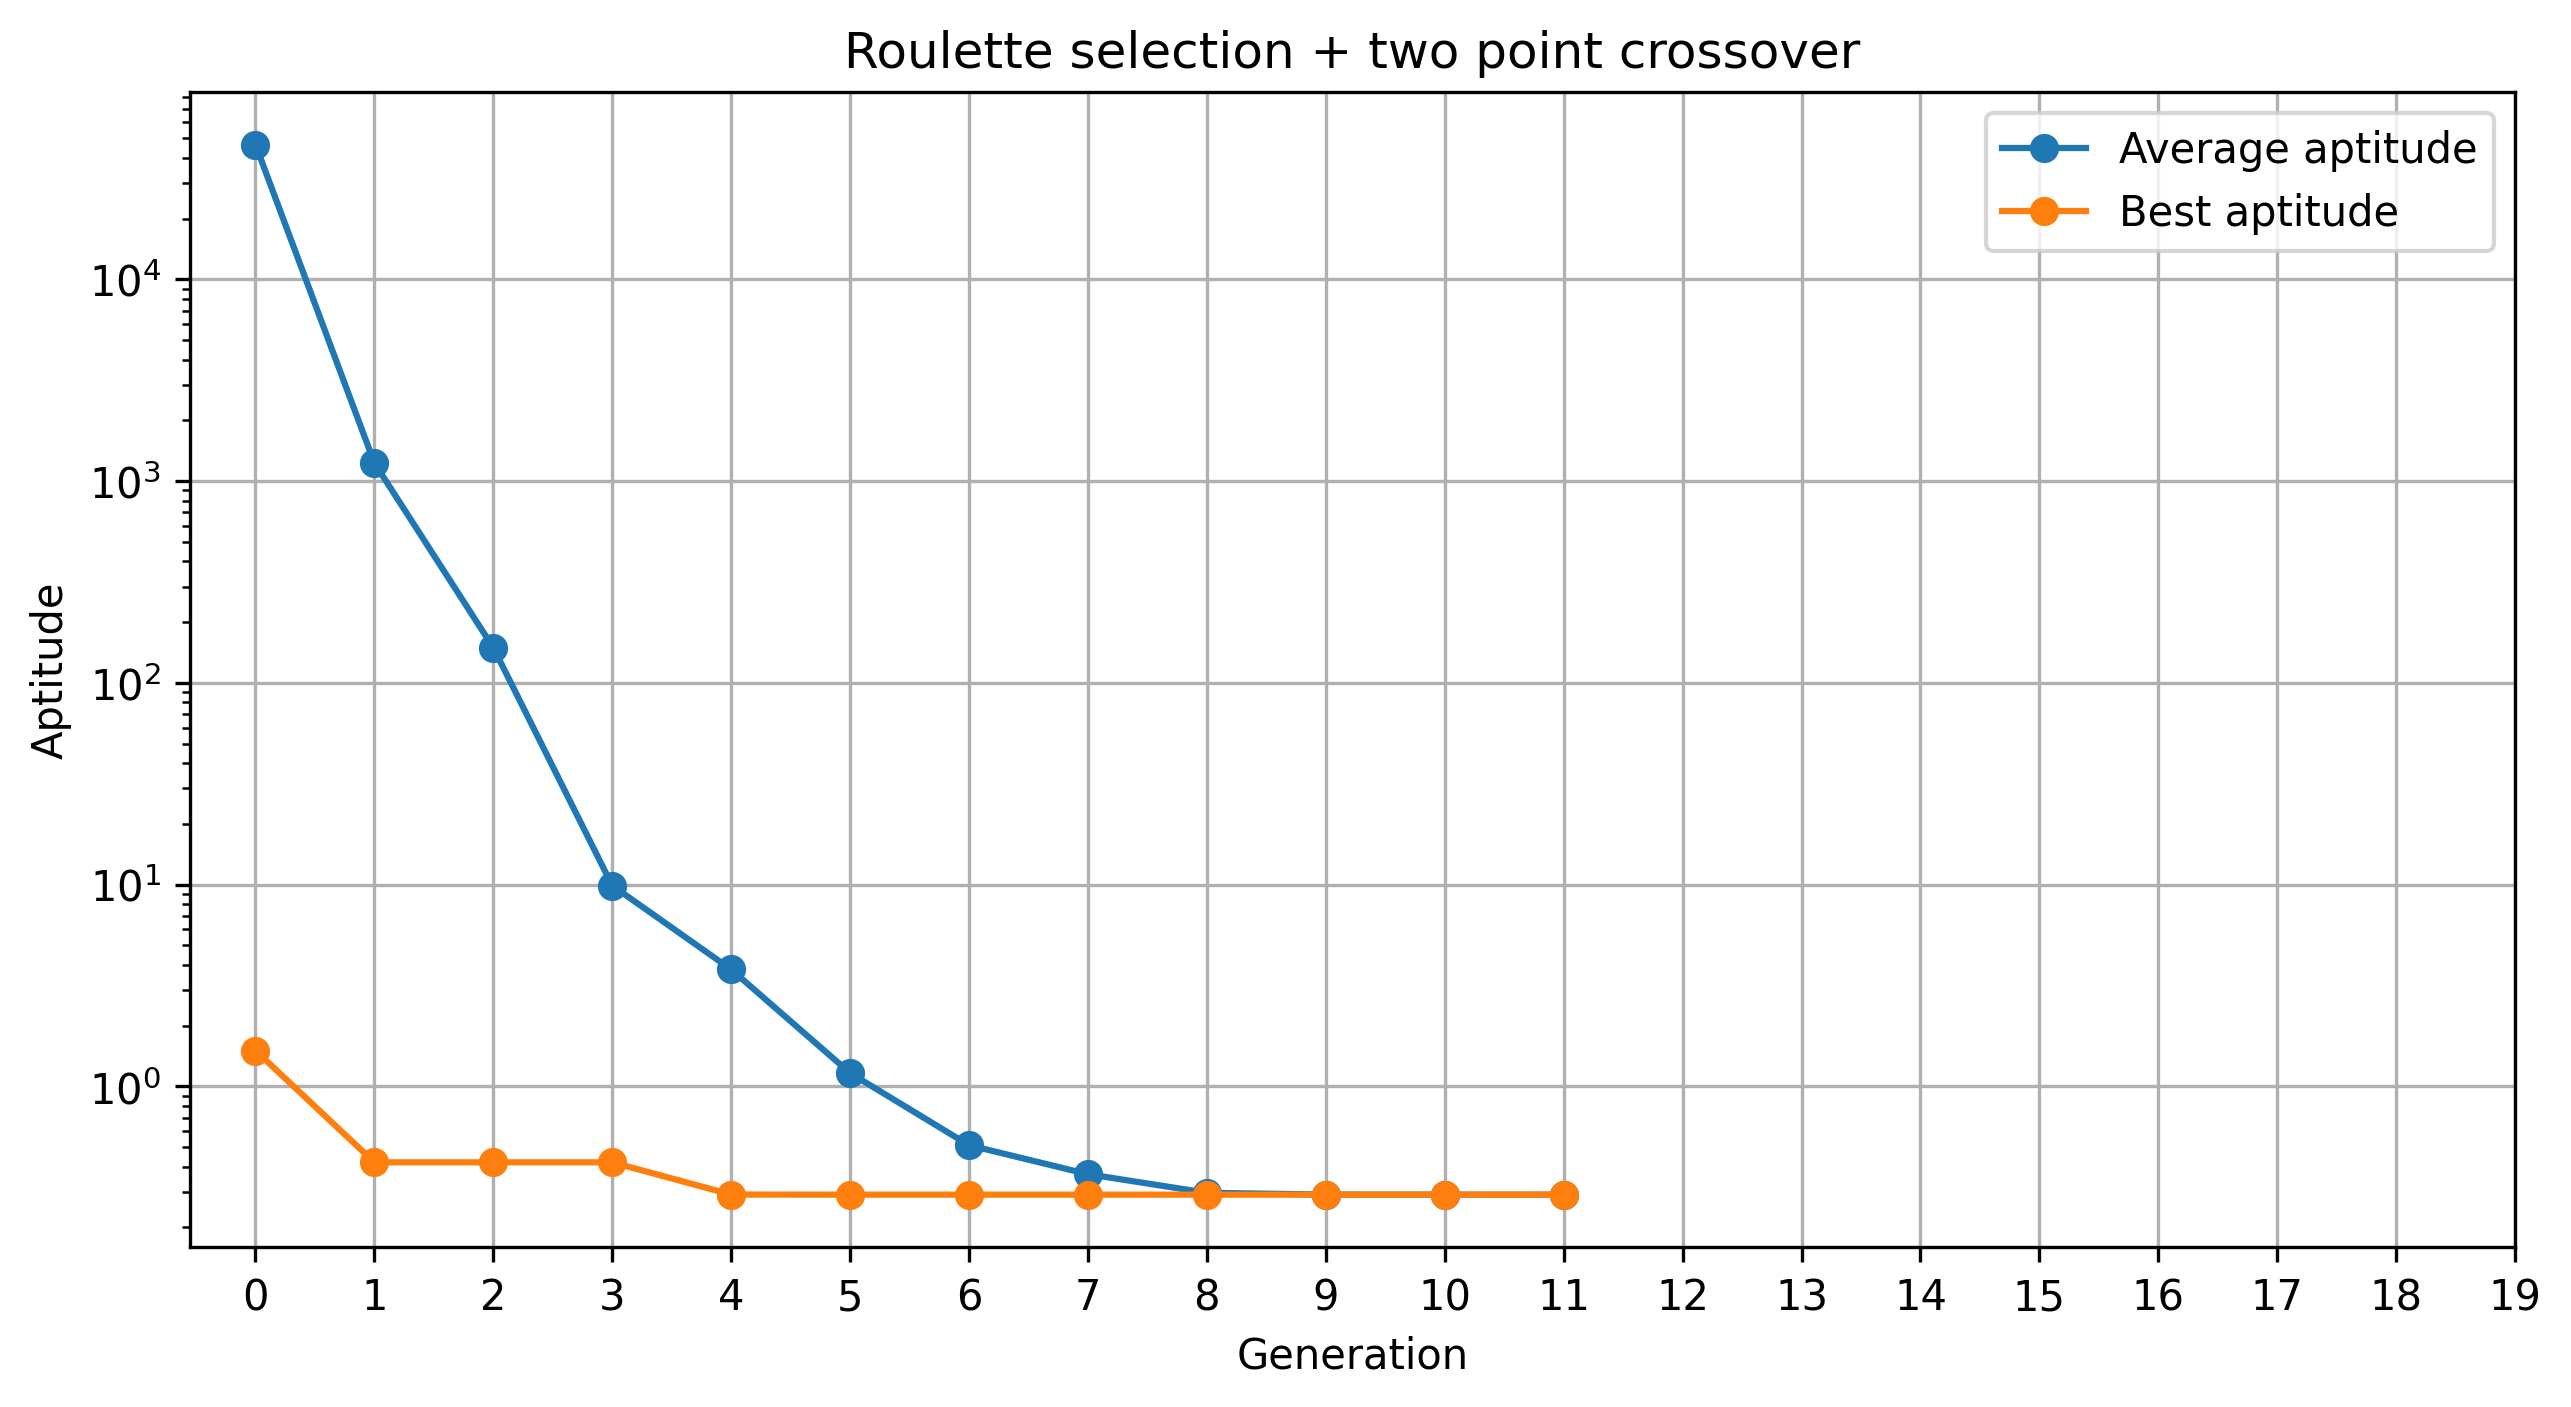
\includegraphics[width=0.7\textwidth]{roulette_selection_two_point_crossover}
	\caption{Evolución de la aptitud de los individuos en primer ejecución.}
	\label{fig:AG_1}
\end{figure}

\begin{figure}
     \centering
     \begin{subfigure}[b]{0.45\textwidth}
         \centering
         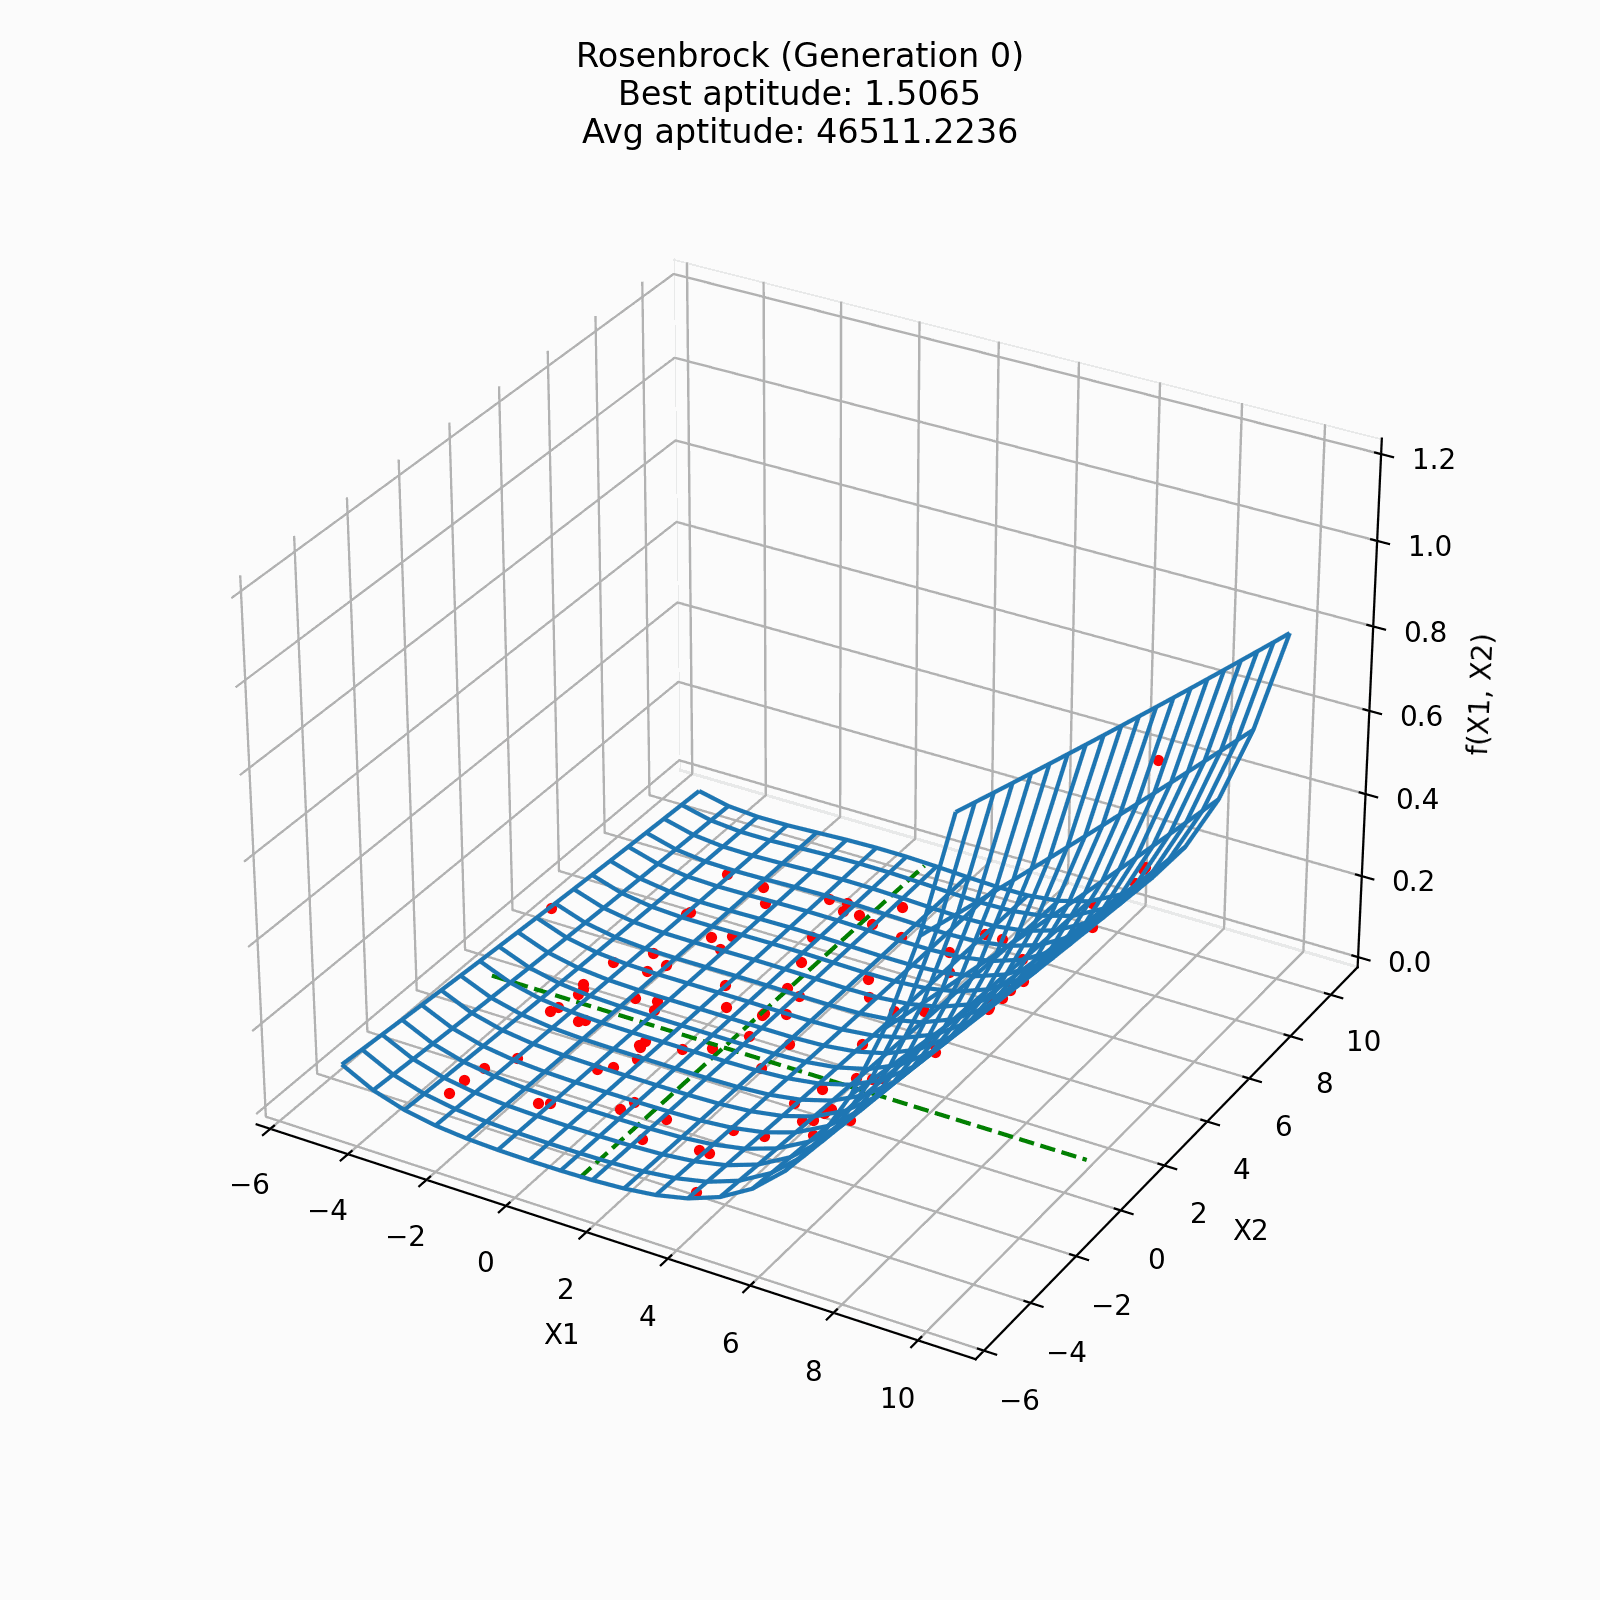
\includegraphics[width=\textwidth]{roulette_selection_two_point_crossover_init}
         \caption{Individuos en la primer época.}
         \label{fig:Ev1_i}
     \end{subfigure}
     \hfill
     \begin{subfigure}[b]{0.45\textwidth}
         \centering
         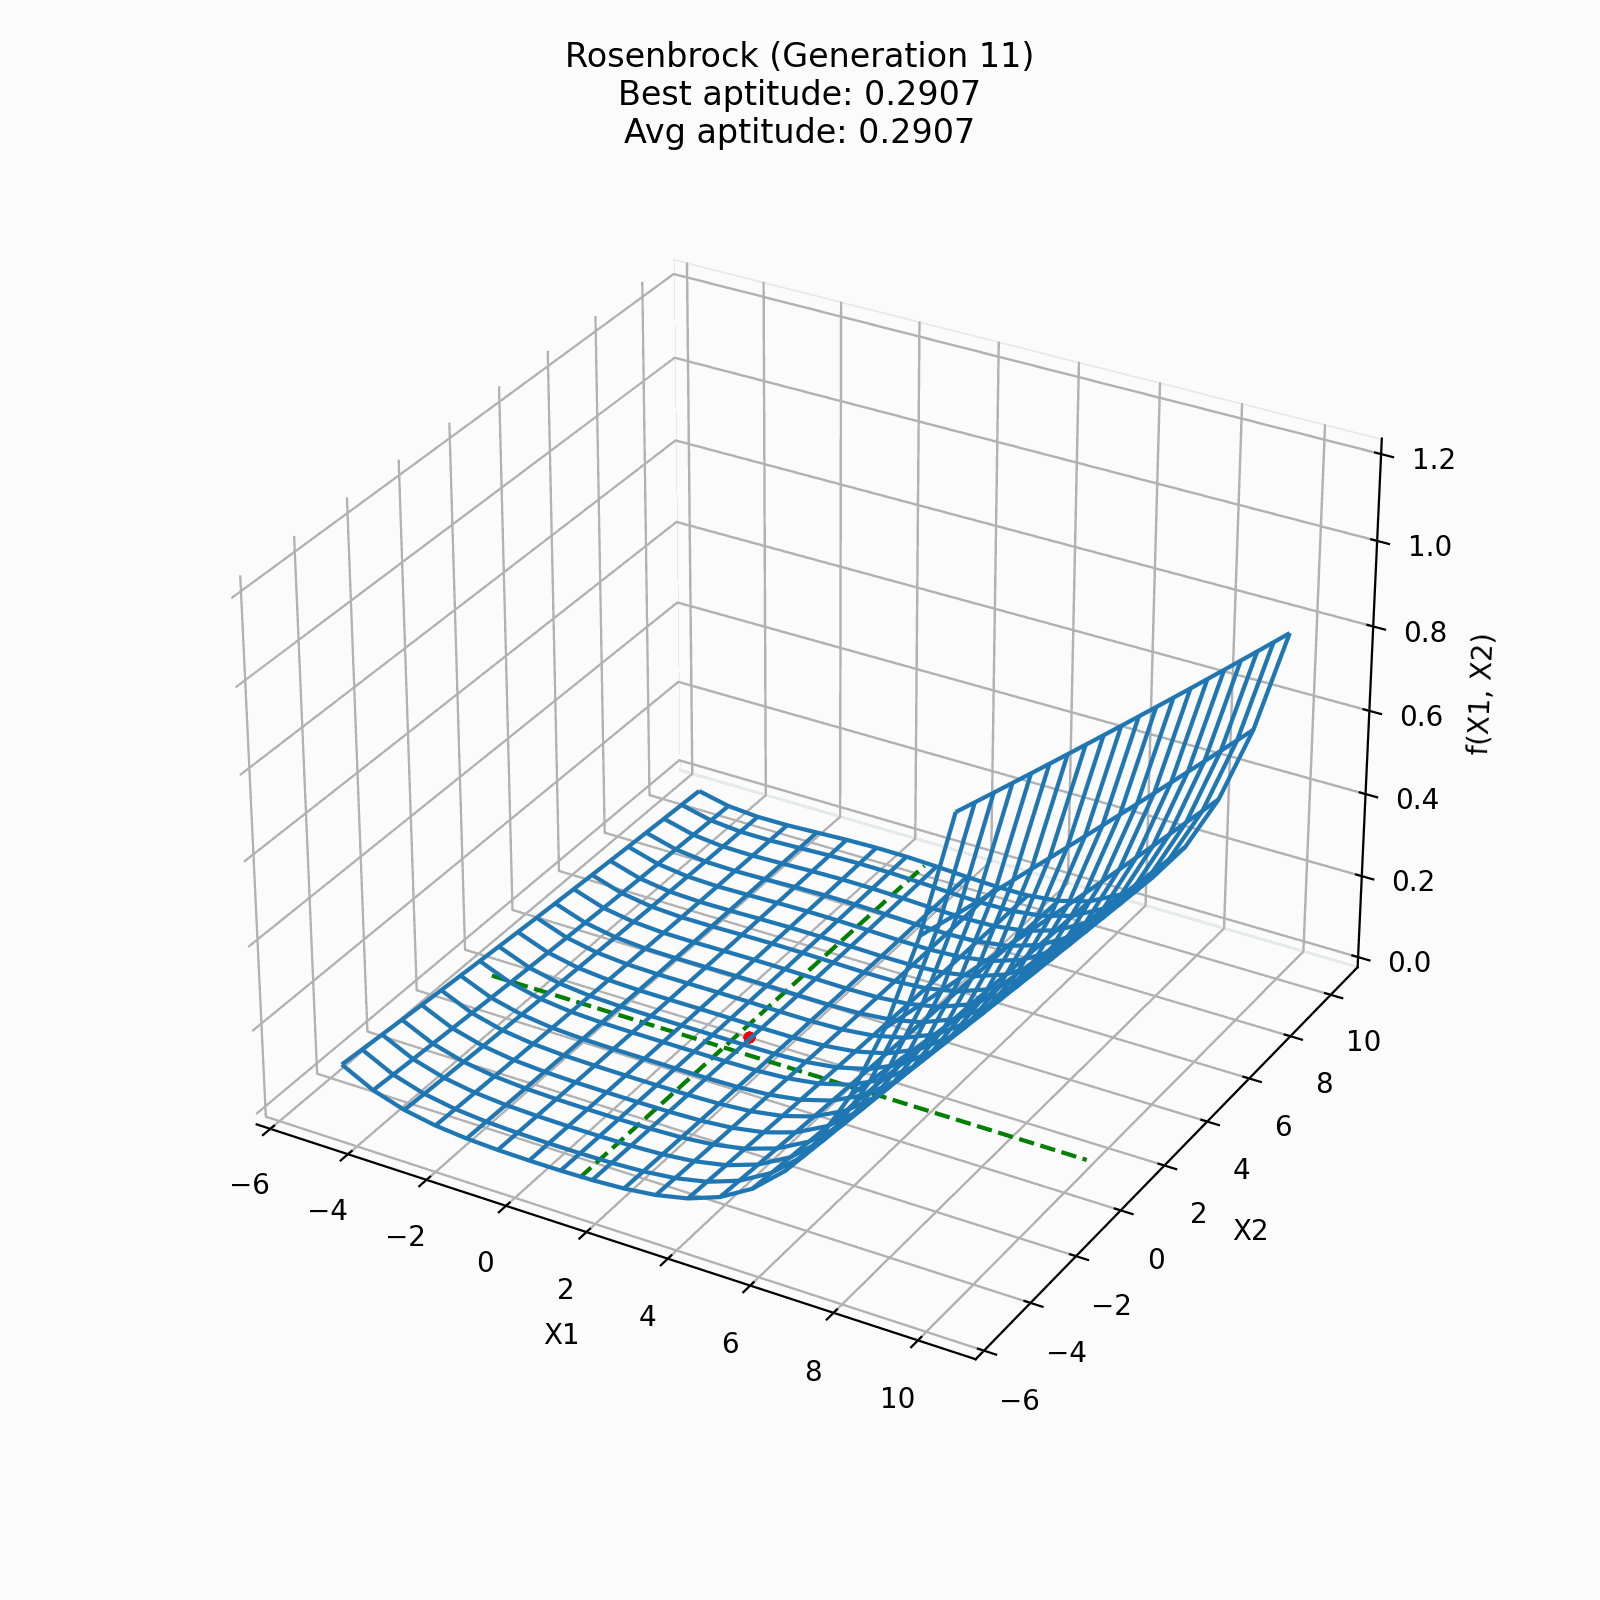
\includegraphics[width=\textwidth]{roulette_selection_two_point_crossover_last}
         \caption{Individuos en la última época.}
         \label{fig:Ev1_f}
     \end{subfigure}
     \caption{Comparación de los individuos entre la primer y última época de la primer ejecución del algoritmo.}
     \label{fig:Ev1}
\end{figure}

\FloatBarrier
Relacionado a la segunda ejecución del algoritmo, este tomó un total de 10 épocas para lograr la convergencia, obteniendo los siguientes resultados:
\begin{itemize}
	\item Mejor individuo: $(1.3542, 1.8367)$
	\item Aptitud: $0.1262$
\end{itemize}

La Figura \ref{fig:AG_2} muestra el proceso de evolución en términos de aptitud, mientras que la Figura \ref{fig:Ev2} muestra una comparación entre los individuos durante la primer época contra los individuos de la última época.

\begin{figure}[htbp]
	\centering
	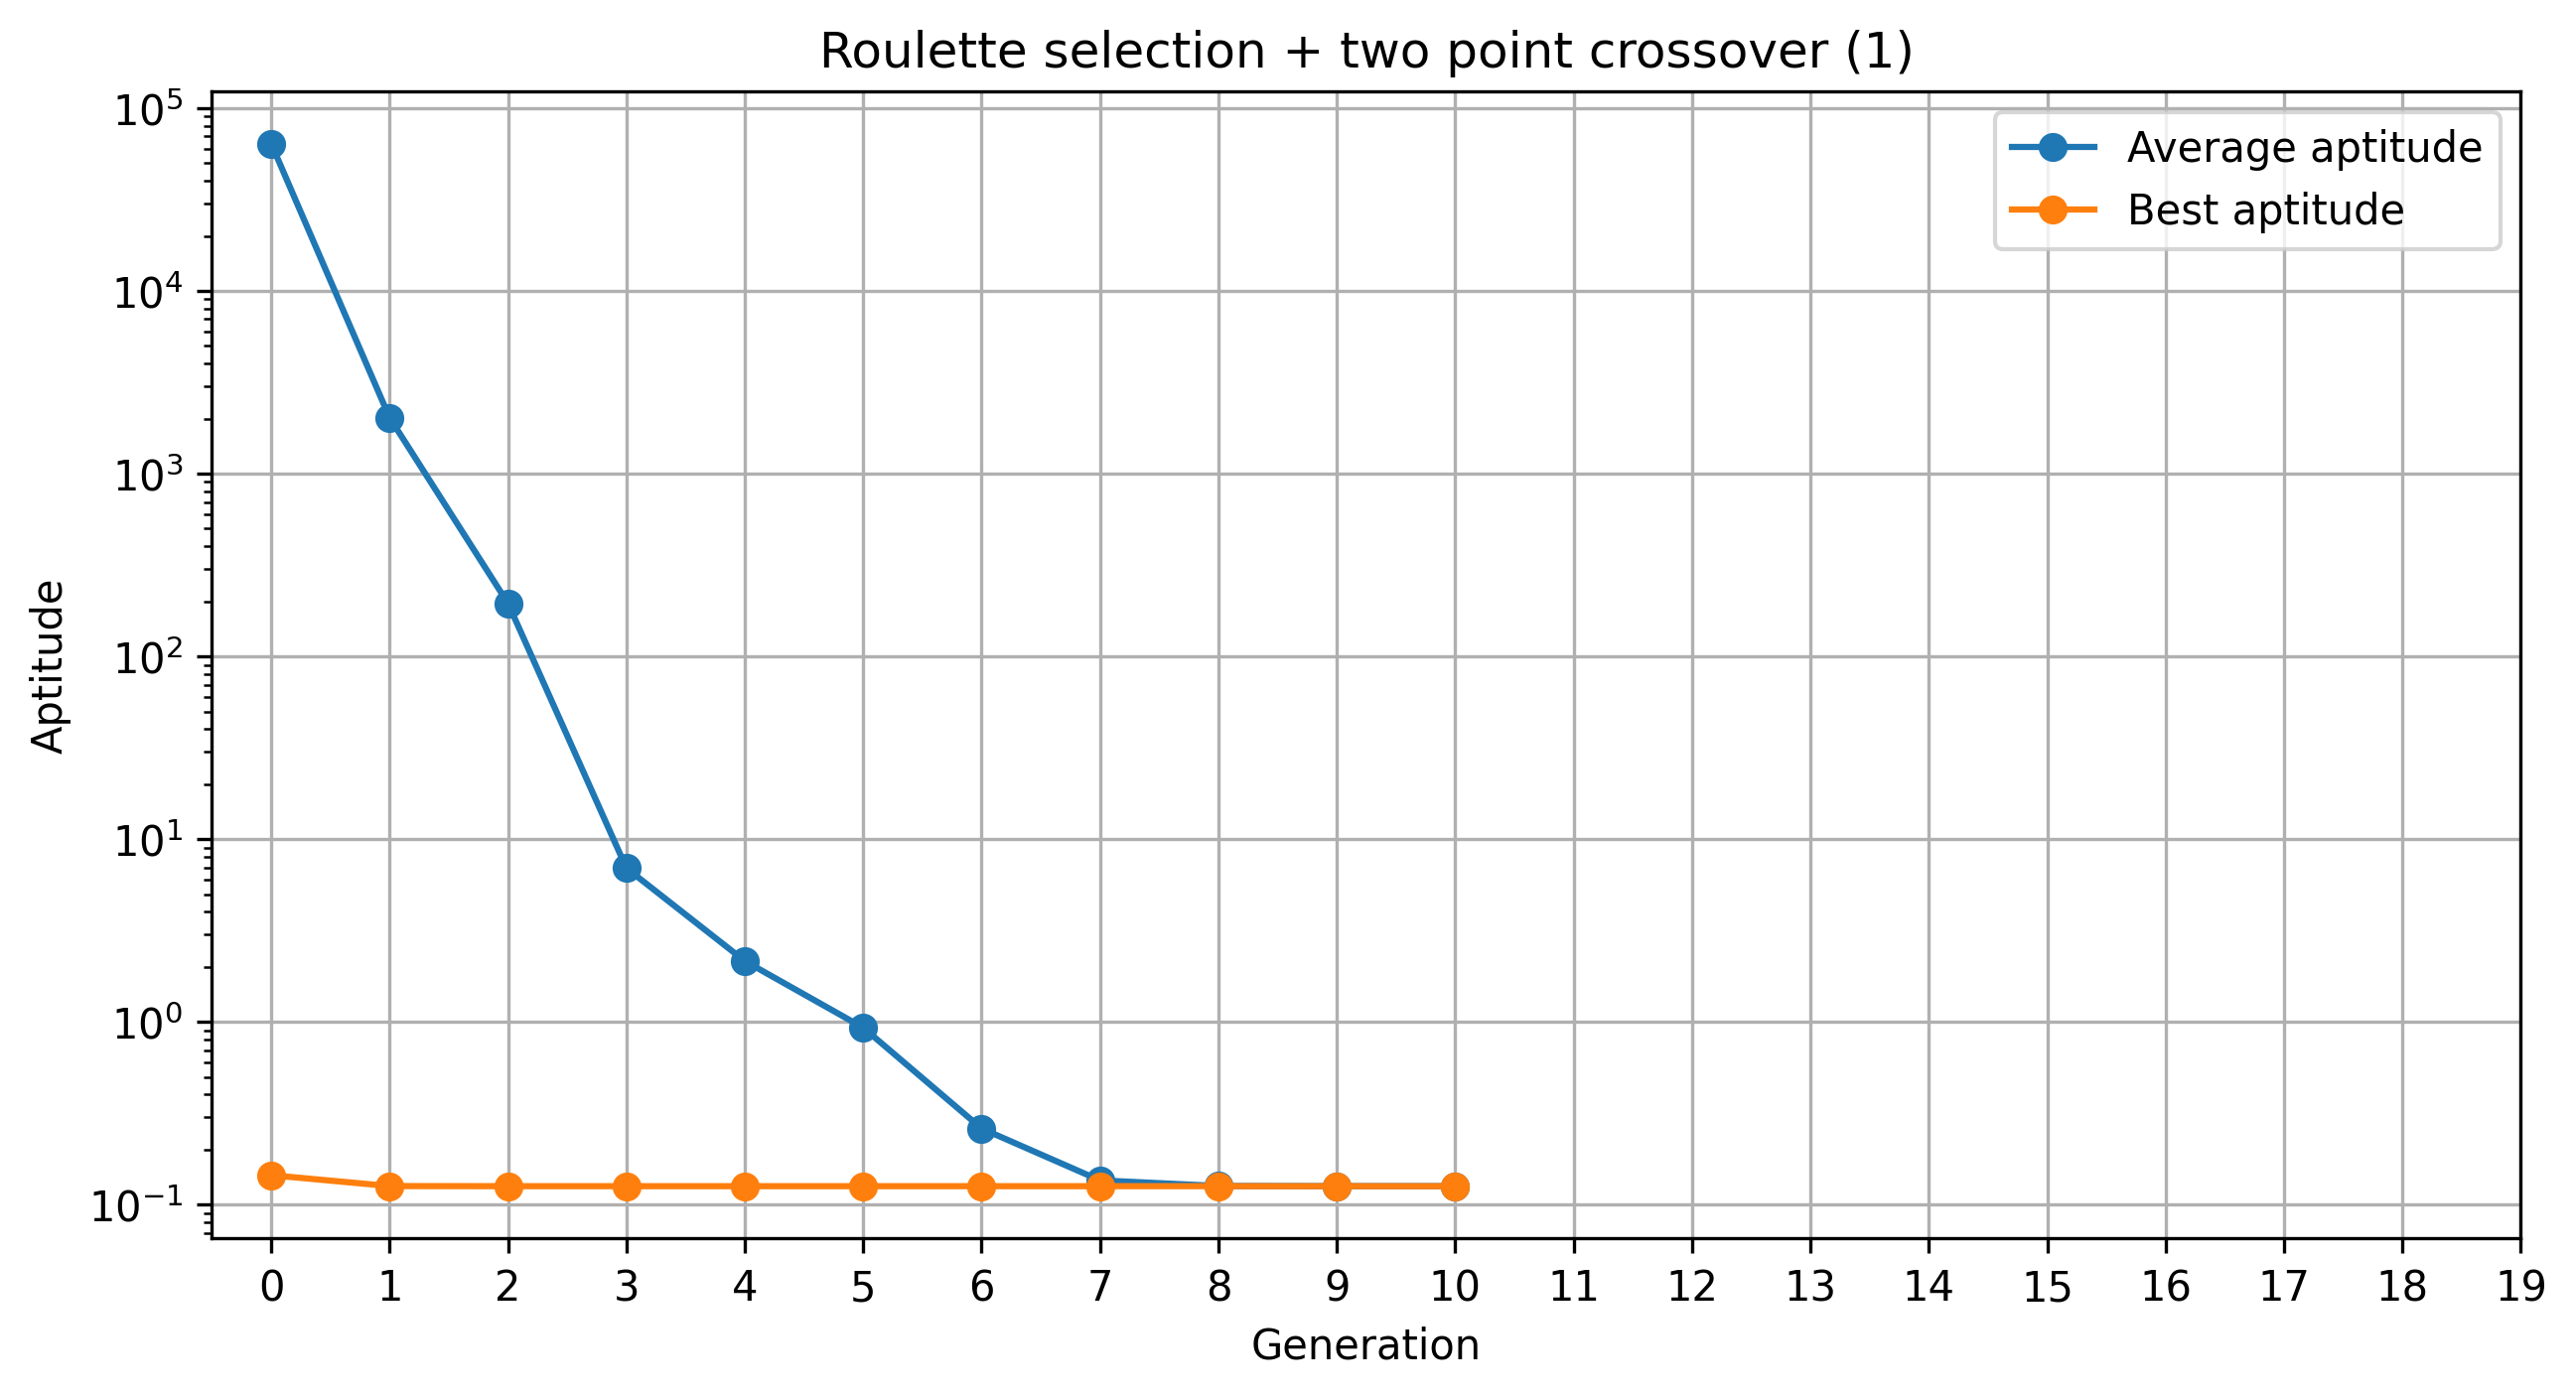
\includegraphics[width=0.7\textwidth]{roulette_selection_two_point_crossover_(1)}
	\caption{Evolución de la aptitud de los individuos en segunda ejecución.}
	\label{fig:AG_2}
\end{figure}

\begin{figure}
     \centering
     \begin{subfigure}[b]{0.45\textwidth}
         \centering
         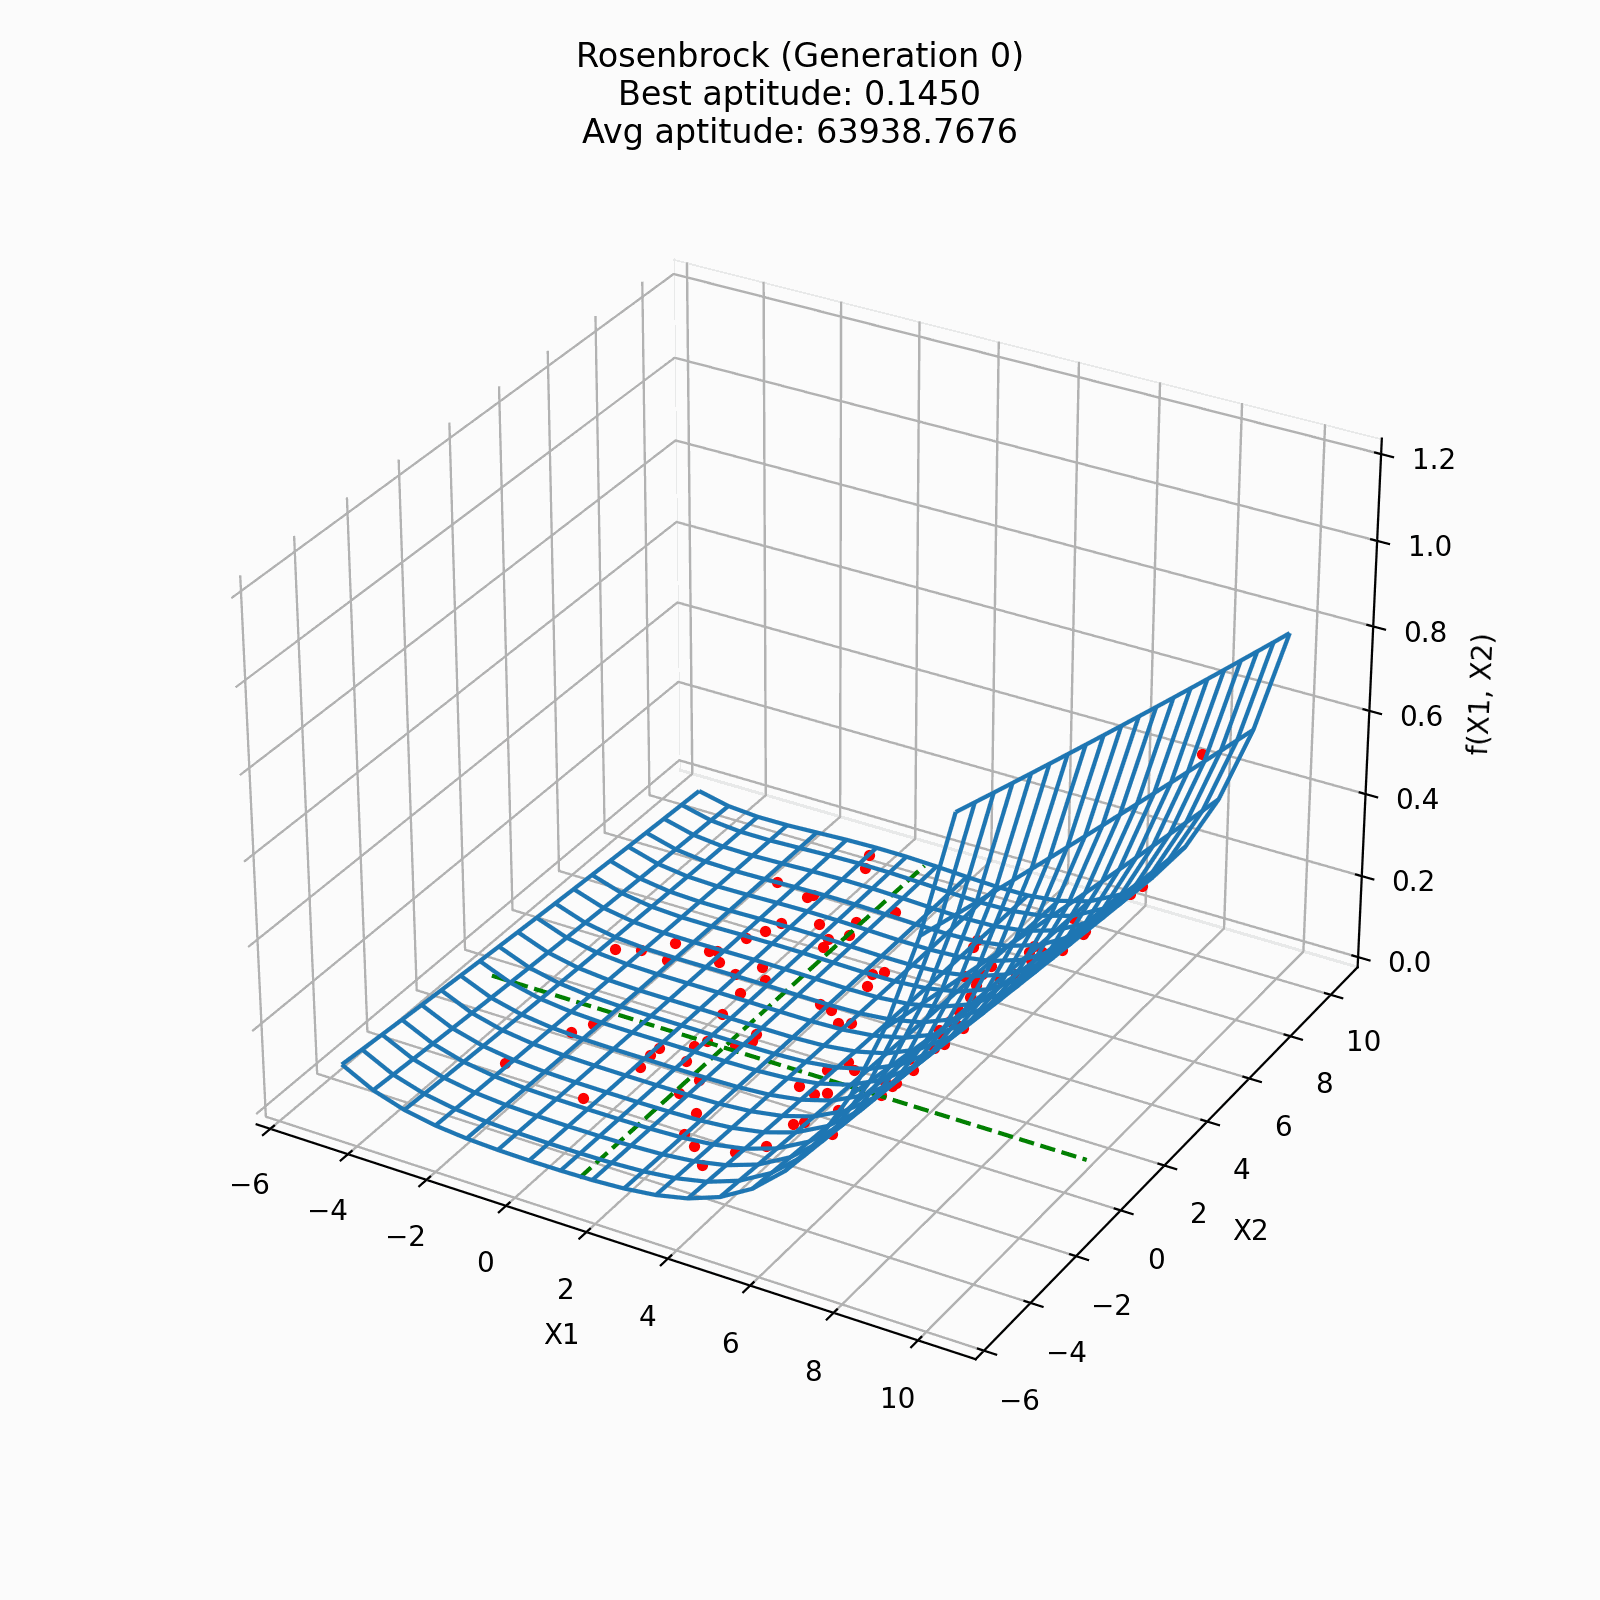
\includegraphics[width=\textwidth]{roulette_selection_two_point_crossover_(1)_init}
         \caption{Individuos en la primer época.}
         \label{fig:Ev2_i}
     \end{subfigure}
     \hfill
     \begin{subfigure}[b]{0.45\textwidth}
         \centering
         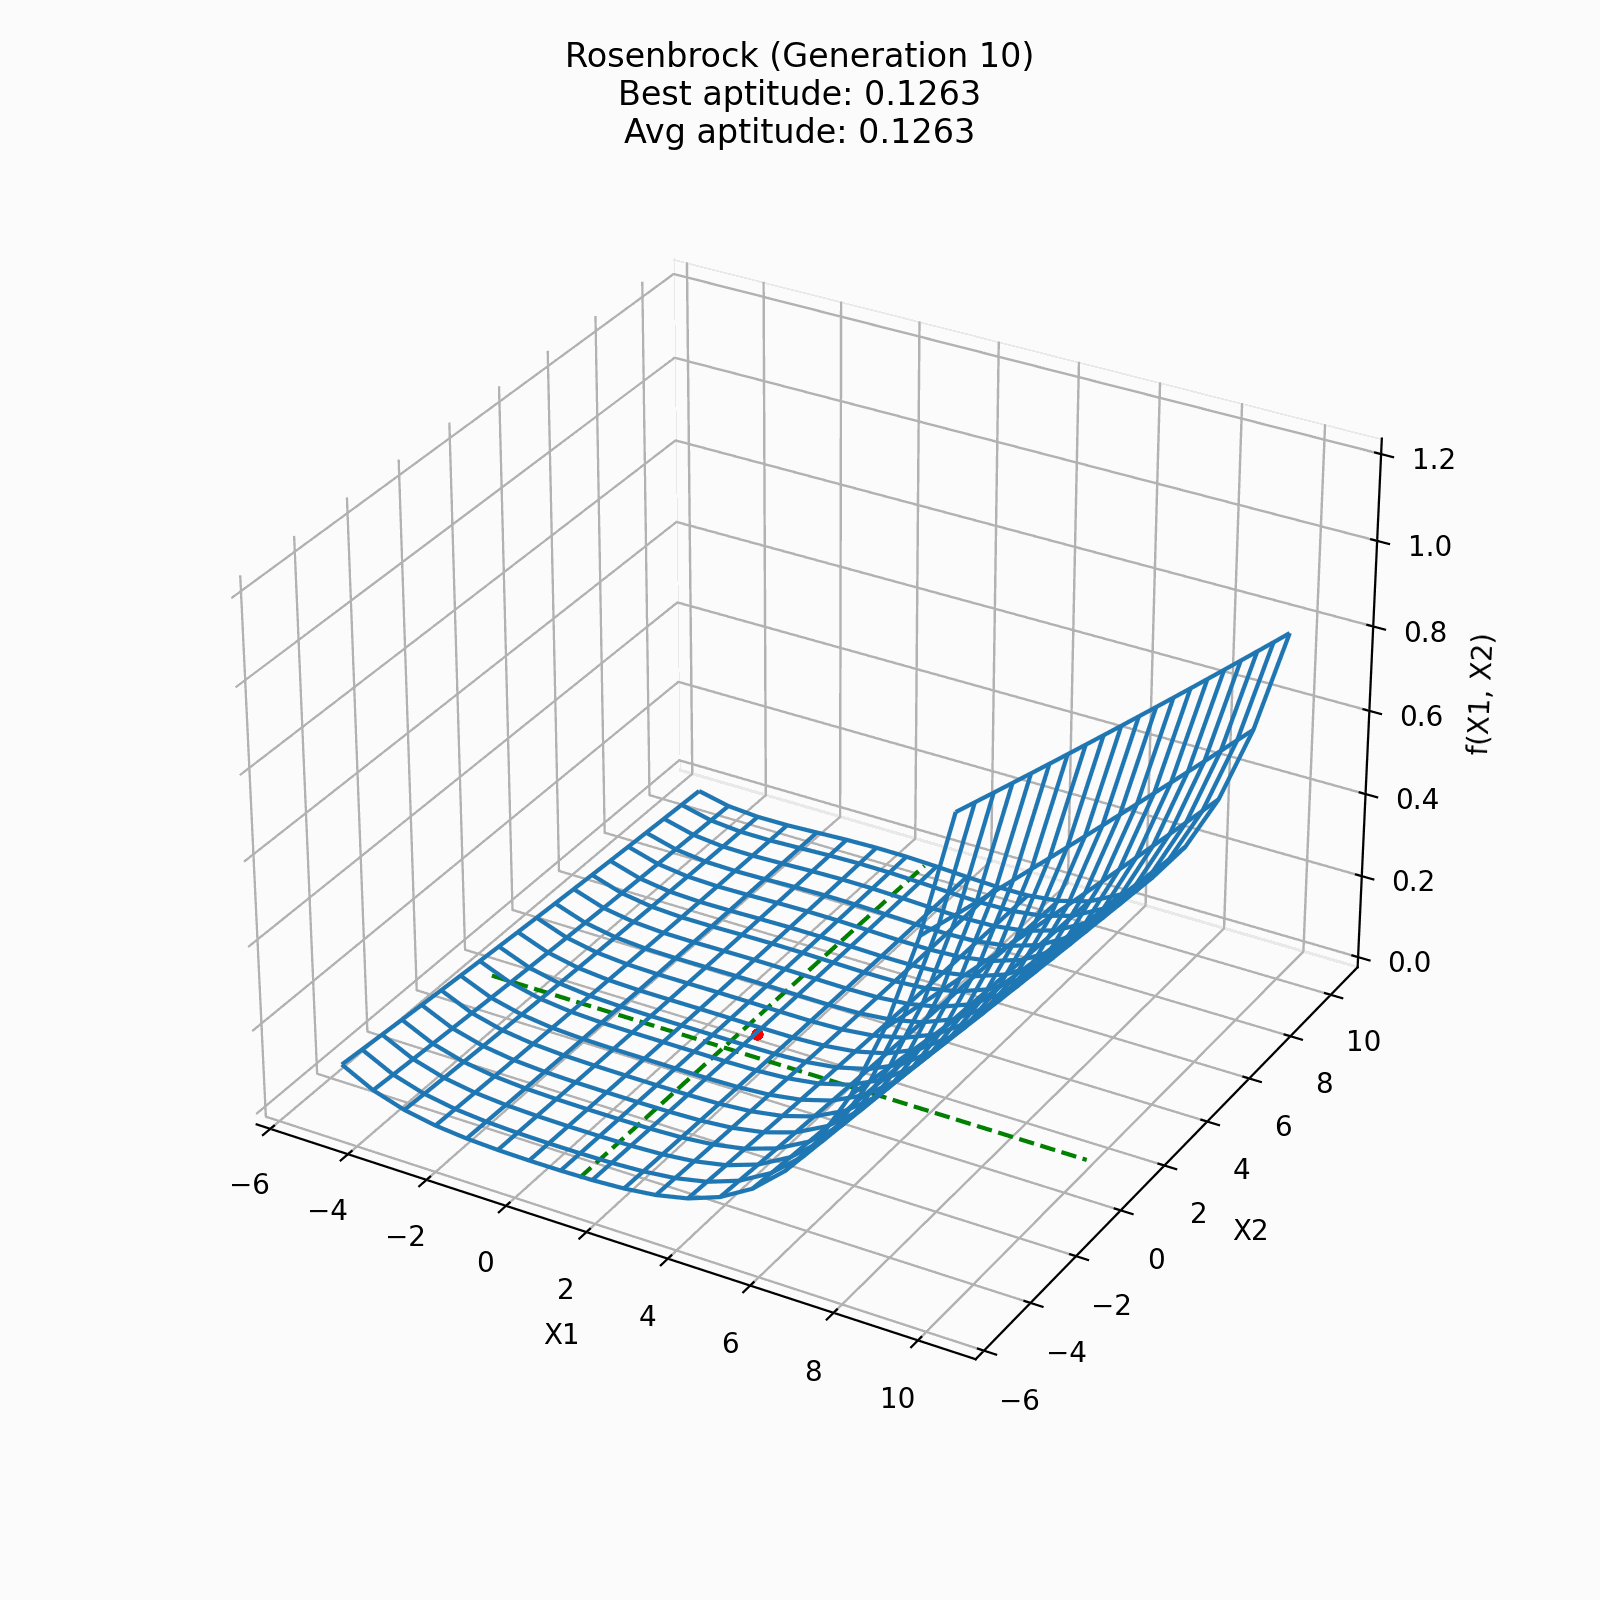
\includegraphics[width=\textwidth]{roulette_selection_two_point_crossover_(1)_last}
         \caption{Individuos en la última época.}
         \label{fig:Ev2_f}
     \end{subfigure}
     \caption{Comparación de los individuos entre la primer y última época de la segunda ejecución del algoritmo.}
     \label{fig:Ev2}
\end{figure}

\FloatBarrier
Relacionado a la tercera ejecución del algoritmo, este tomó un total de 11 épocas para lograr la convergencia, obteniendo los siguientes resultados:
\begin{itemize}
	\item Mejor individuo: $(0.8287, 0.7170)$
	\item Aptitud: $0.1203$
\end{itemize}

La Figura \ref{fig:AG_3} muestra el proceso de evolución en términos de aptitud, mientras que la Figura \ref{fig:Ev3} muestra una comparación entre los individuos durante la primer época contra los individuos de la última época.

\begin{figure}[htbp]
	\centering
	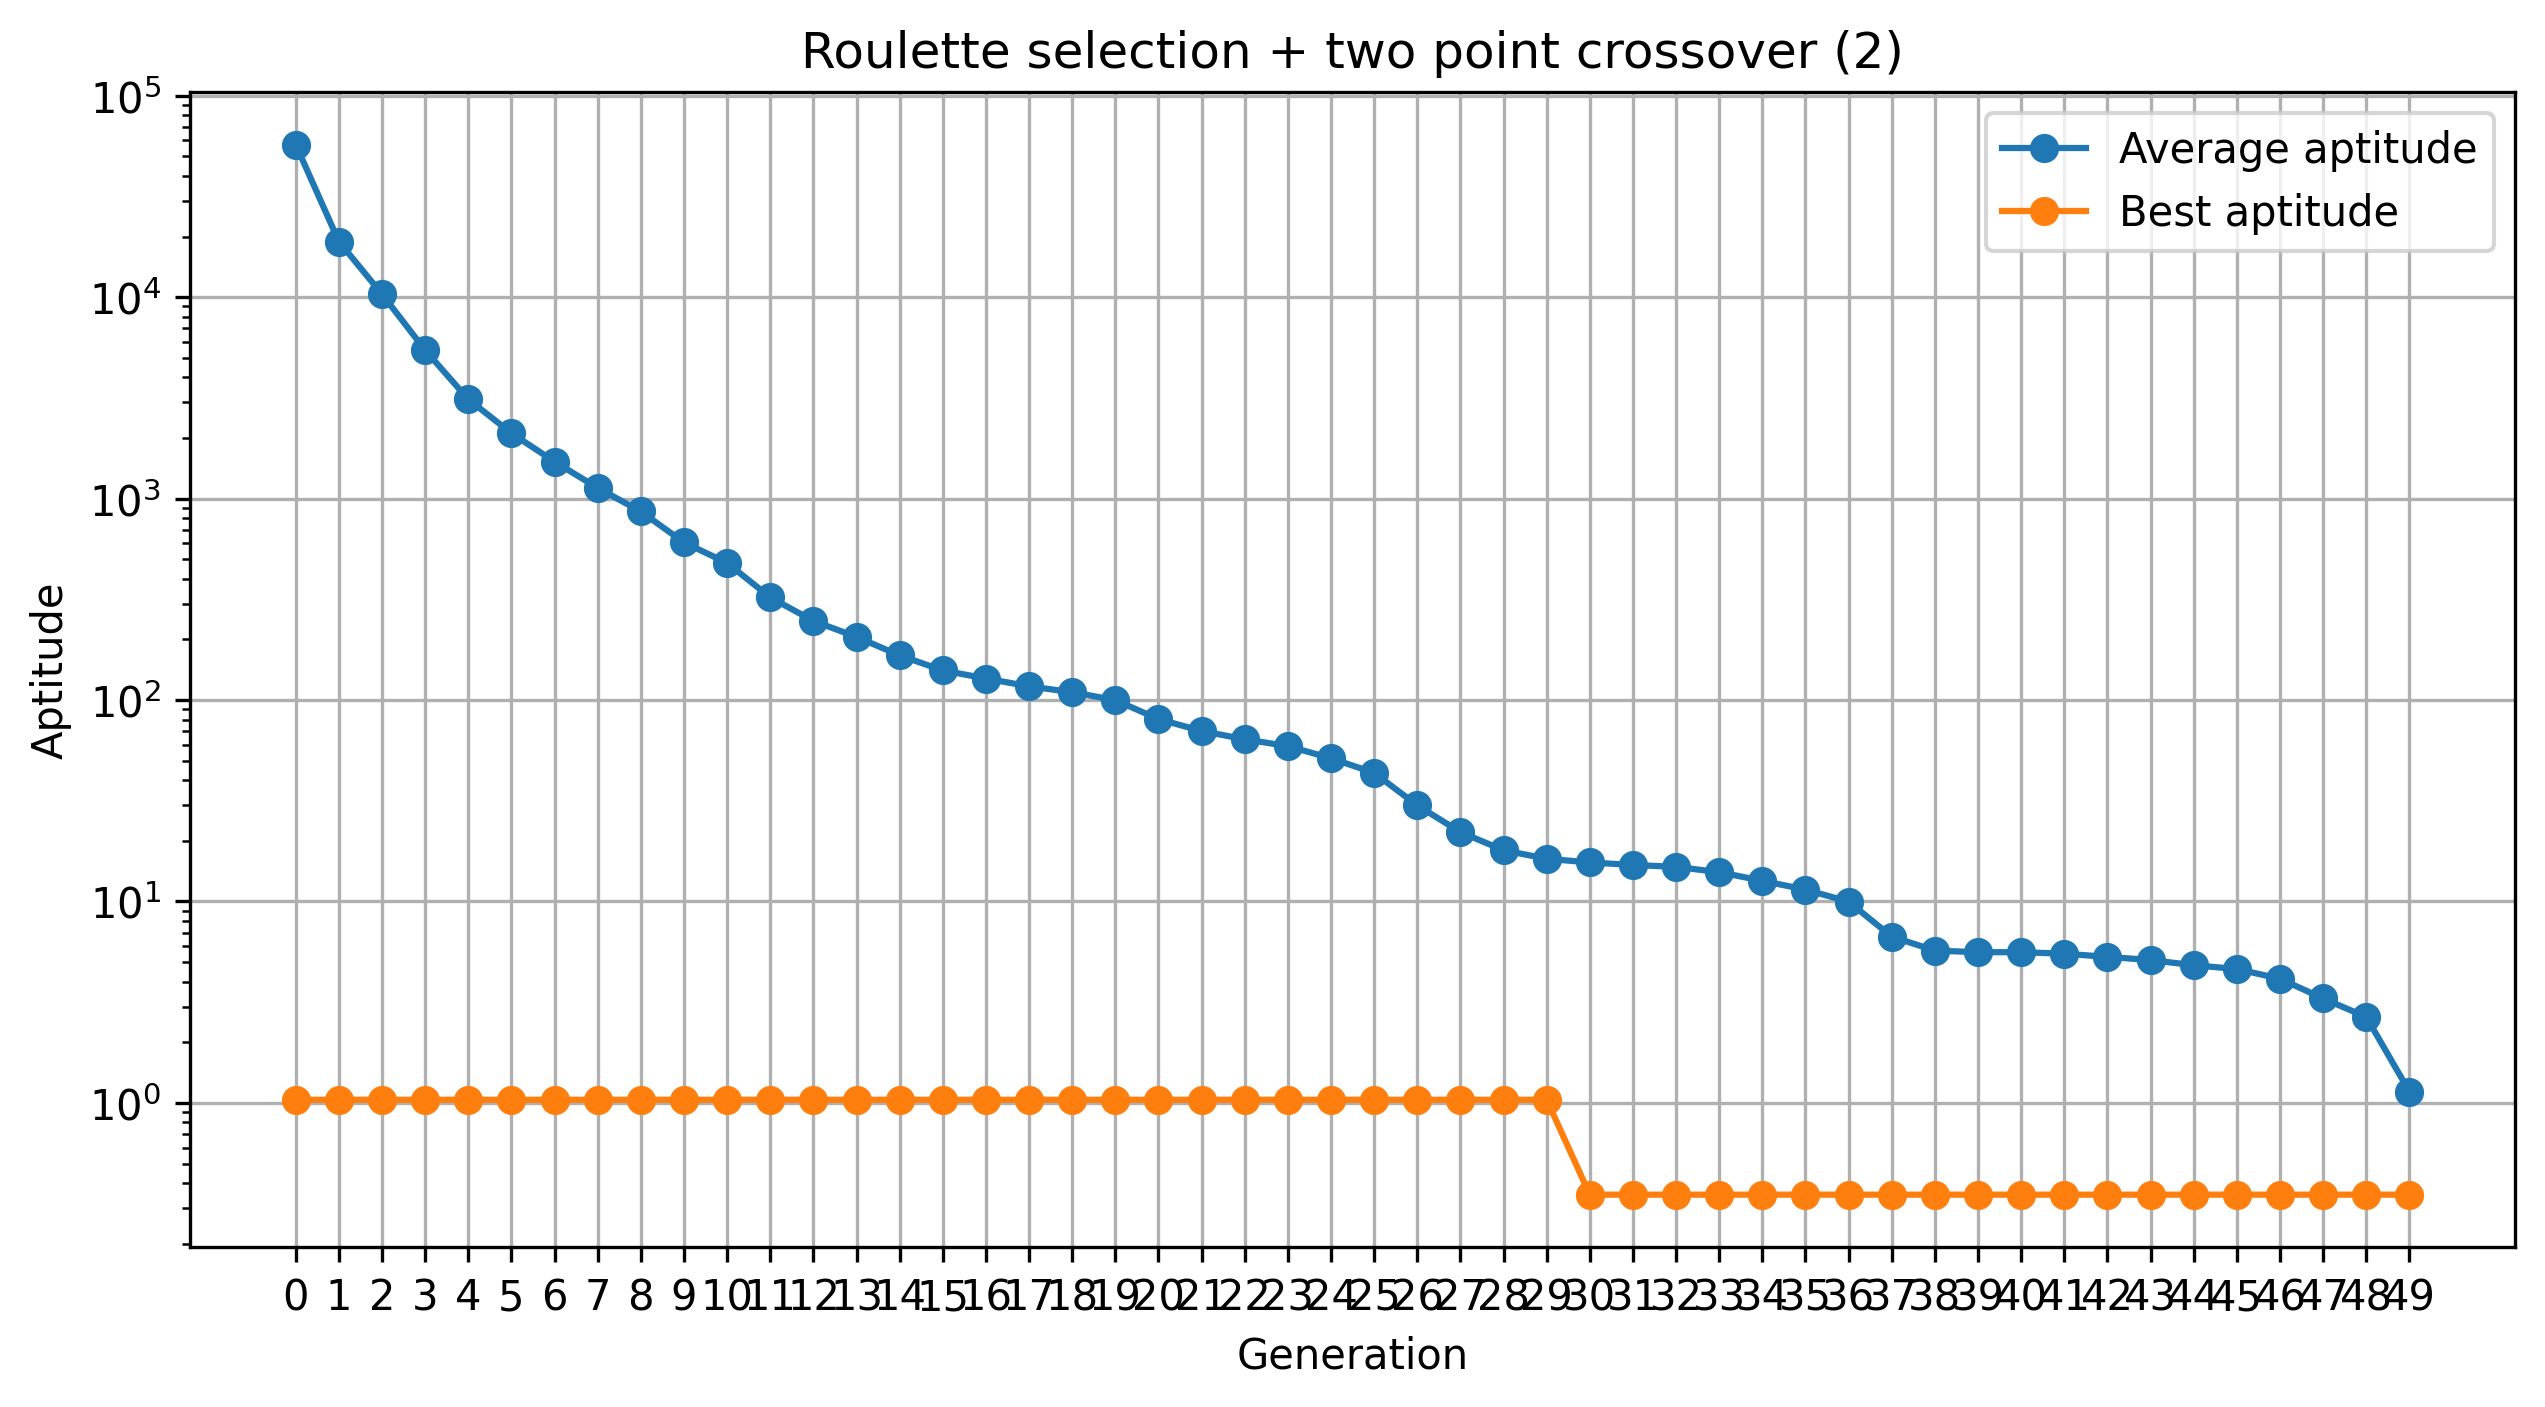
\includegraphics[width=0.7\textwidth]{roulette_selection_two_point_crossover_(2)}
	\caption{Evolución de la aptitud de los individuos en tercera ejecución.}
	\label{fig:AG_3}
\end{figure}

\begin{figure}
     \centering
     \begin{subfigure}[b]{0.45\textwidth}
         \centering
         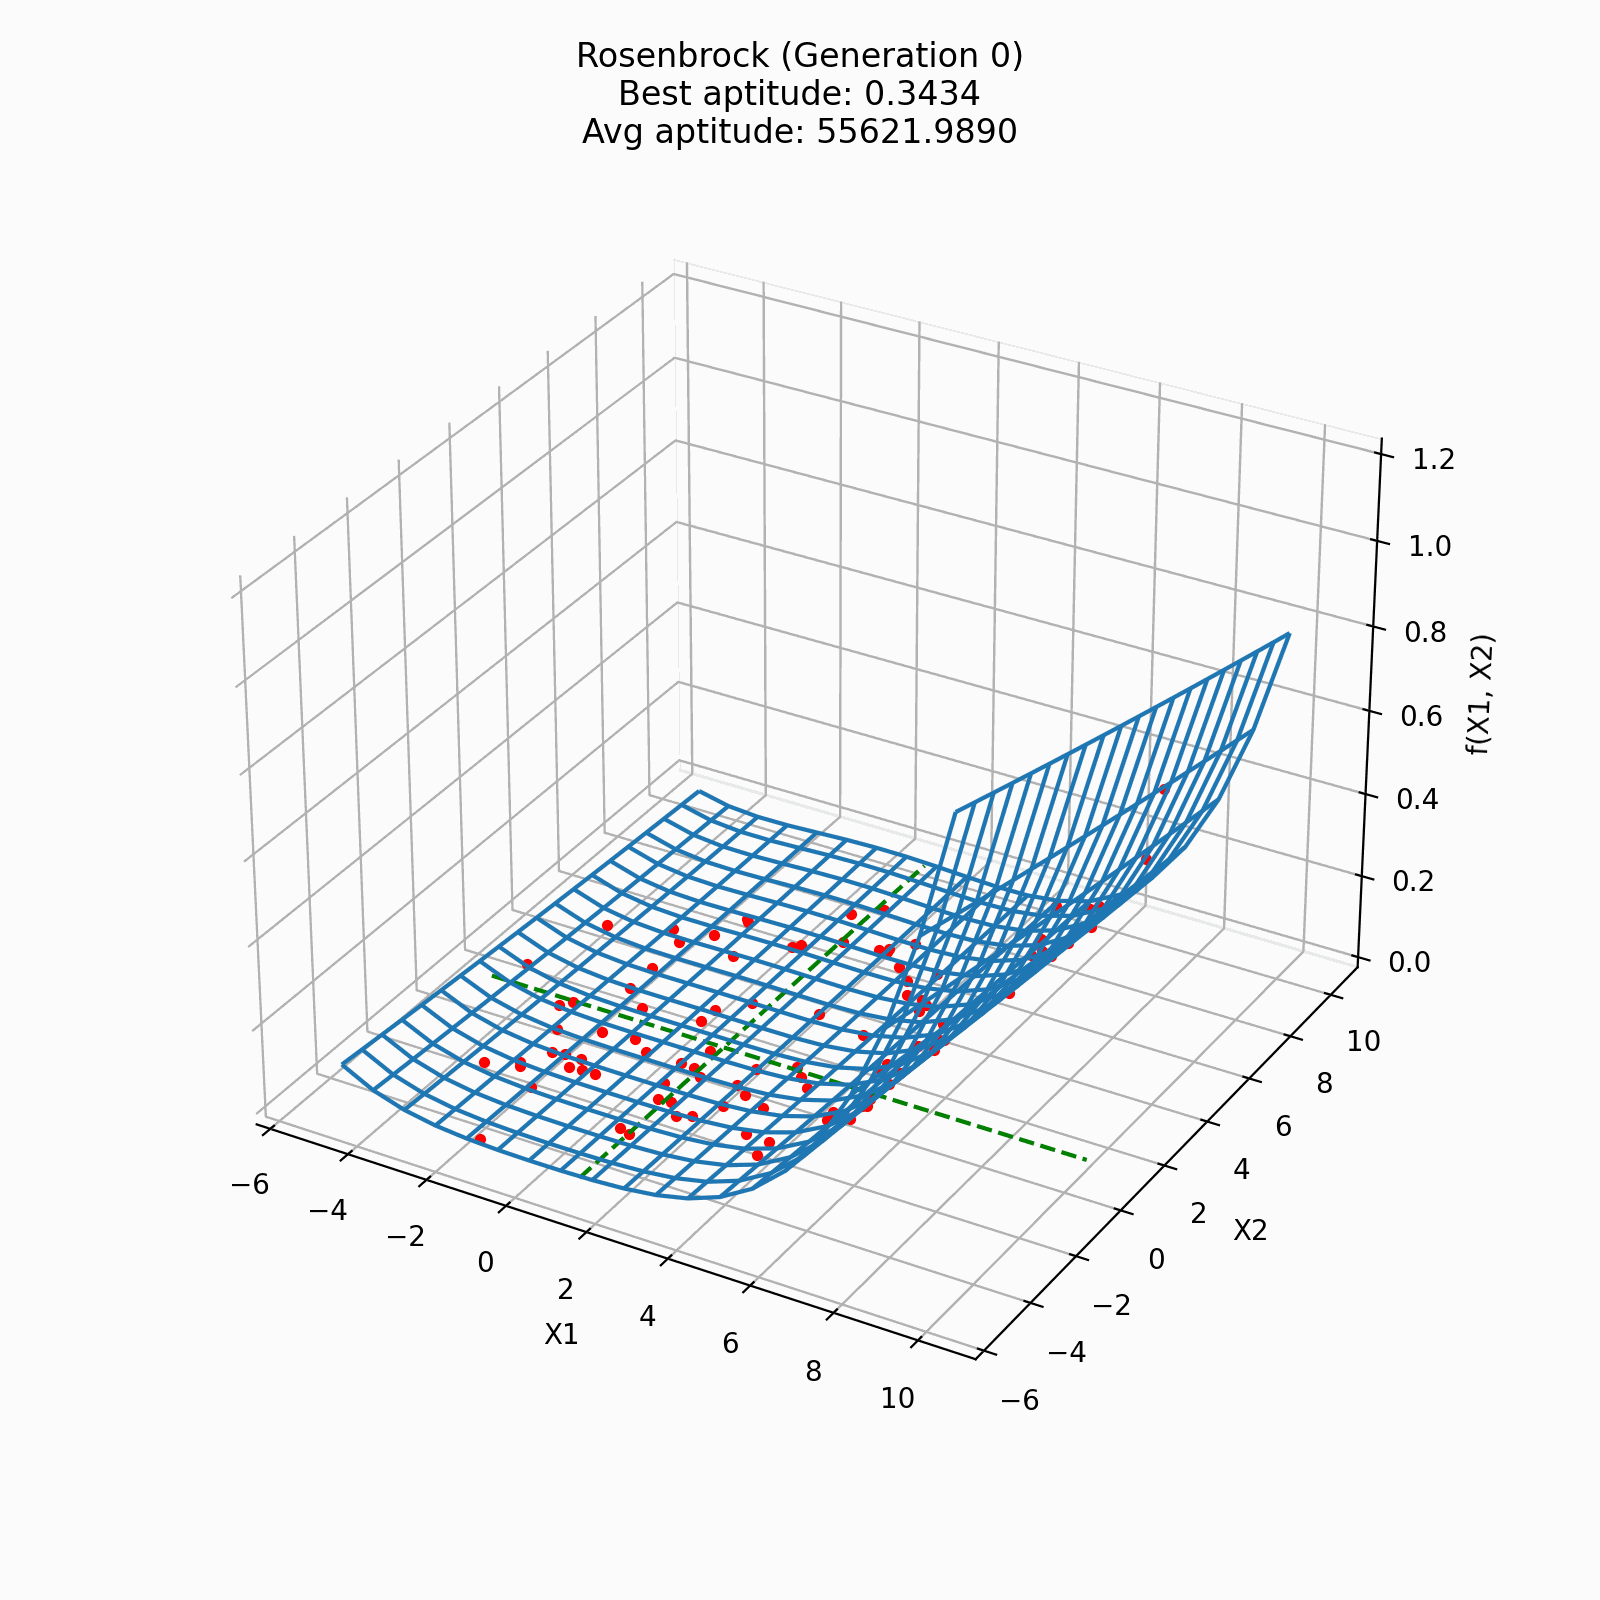
\includegraphics[width=\textwidth]{roulette_selection_two_point_crossover_(2)_init}
         \caption{Individuos en la primer época.}
         \label{fig:Ev3_i}
     \end{subfigure}
     \hfill
     \begin{subfigure}[b]{0.45\textwidth}
         \centering
         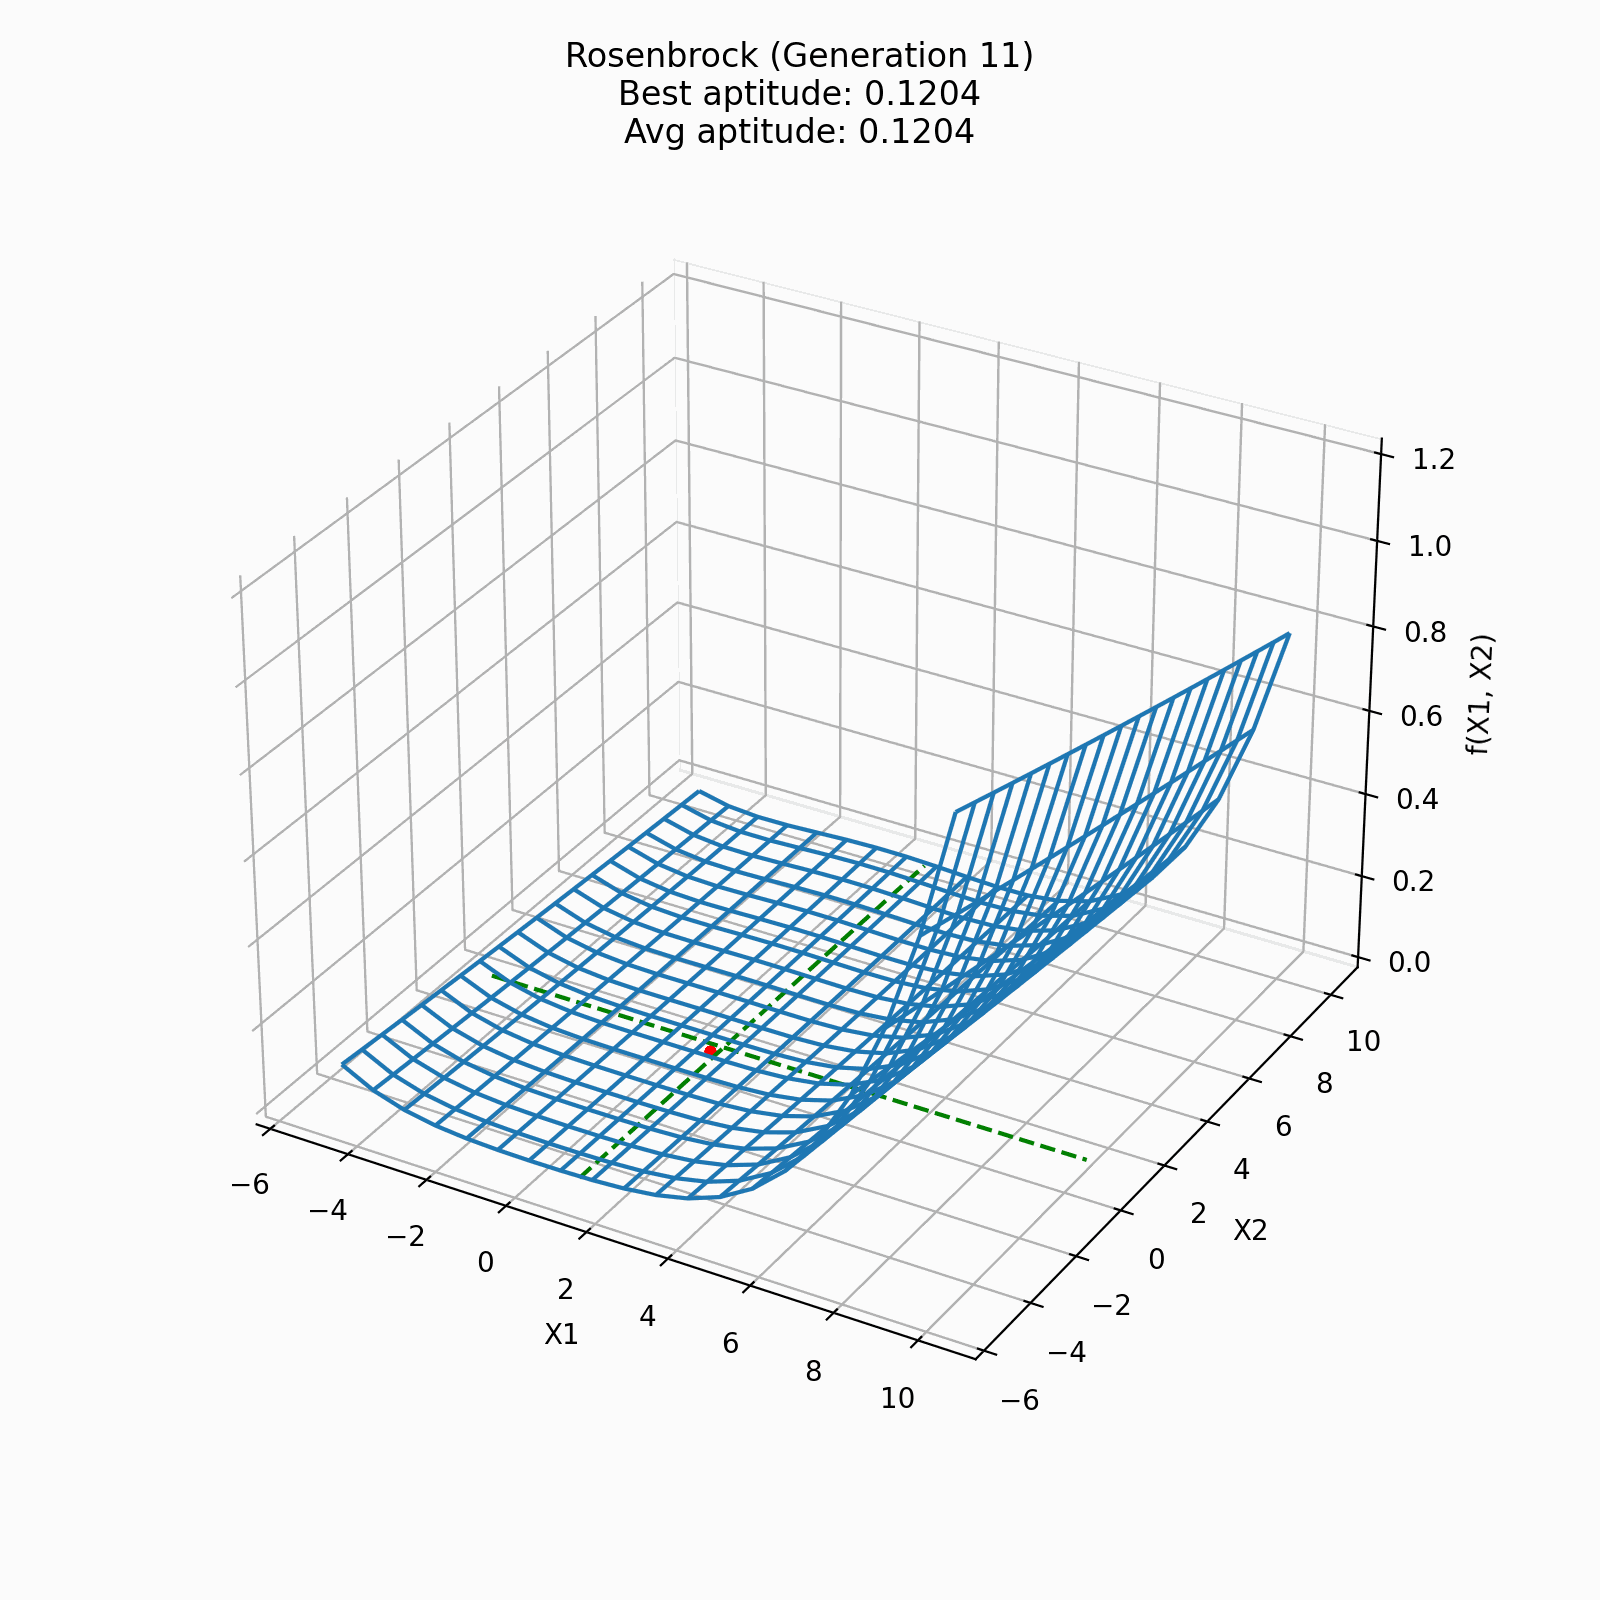
\includegraphics[width=\textwidth]{roulette_selection_two_point_crossover_(2)_last}
         \caption{Individuos en la última época.}
         \label{fig:Ev3_f}
     \end{subfigure}
     \caption{Comparación de los individuos entre la primer y última época de la tercera ejecución del algoritmo.}
     \label{fig:Ev3}
\end{figure}
